\documentclass[]{elsarticle} %review=doublespace preprint=single 5p=2 column
%%% Begin My package additions %%%%%%%%%%%%%%%%%%%
\usepackage[hyphens]{url}

  \journal{Transportation Research Part D: Transport and Environment} % Sets Journal name


\usepackage{lineno} % add
\providecommand{\tightlist}{%
  \setlength{\itemsep}{0pt}\setlength{\parskip}{0pt}}

\usepackage{graphicx}
\usepackage{booktabs} % book-quality tables
%%%%%%%%%%%%%%%% end my additions to header

\usepackage[T1]{fontenc}
\usepackage{lmodern}
\usepackage{amssymb,amsmath}
\usepackage{ifxetex,ifluatex}
\usepackage{fixltx2e} % provides \textsubscript
% use upquote if available, for straight quotes in verbatim environments
\IfFileExists{upquote.sty}{\usepackage{upquote}}{}
\ifnum 0\ifxetex 1\fi\ifluatex 1\fi=0 % if pdftex
  \usepackage[utf8]{inputenc}
\else % if luatex or xelatex
  \usepackage{fontspec}
  \ifxetex
    \usepackage{xltxtra,xunicode}
  \fi
  \defaultfontfeatures{Mapping=tex-text,Scale=MatchLowercase}
  \newcommand{\euro}{€}
\fi
% use microtype if available
\IfFileExists{microtype.sty}{\usepackage{microtype}}{}
\bibliographystyle{elsarticle-harv}
\usepackage{graphicx}
\ifxetex
  \usepackage[setpagesize=false, % page size defined by xetex
              unicode=false, % unicode breaks when used with xetex
              xetex]{hyperref}
\else
  \usepackage[unicode=true]{hyperref}
\fi
\hypersetup{breaklinks=true,
            bookmarks=true,
            pdfauthor={},
            pdftitle={Examining spatial equity and accessibility to a public bicycle share program using a balanced floating catchment area approach},
            colorlinks=false,
            urlcolor=blue,
            linkcolor=magenta,
            pdfborder={0 0 0}}
\urlstyle{same}  % don't use monospace font for urls

\setcounter{secnumdepth}{0}
% Pandoc toggle for numbering sections (defaults to be off)
\setcounter{secnumdepth}{0}

% Pandoc citation processing

% Pandoc header
\usepackage{booktabs}
\usepackage{longtable}
\usepackage{array}
\usepackage{multirow}
\usepackage{wrapfig}
\usepackage{float}
\usepackage{colortbl}
\usepackage{pdflscape}
\usepackage{tabu}
\usepackage{threeparttable}
\usepackage{threeparttablex}
\usepackage[normalem]{ulem}
\usepackage{makecell}
\usepackage{xcolor}



\begin{document}
\begin{frontmatter}

  \title{Examining spatial equity and accessibility to a public bicycle share
program using a balanced floating catchment area approach}
    \author[Some School]{Antonio Paez\corref{1}}
   \ead{paez@mcmaster.ca} 
    \author[Some School]{Elise Desjardins\corref{2}}
   \ead{desjae@mcmaster.ca} 
    \author[Another University]{Christopher D. Higgins\corref{2}}
   \ead{cd.higgins@utoronto.ca} 
      \address[McMaster University]{School of Earth, Environment \& Society, 1280 Main Street West,
Hamilton, ON}
    \address[University of Toronto Scarborough]{Department, Street, City, State, Zip}
      \cortext[1]{Corresponding Author}
    \cortext[2]{Equal contribution}
  
  \begin{abstract}
  This is the abstract.
  
  It consists of two paragraphs.
  \end{abstract}
  
 \end{frontmatter}

\begin{verbatim}
## 
## Attaching package: 'dplyr'
\end{verbatim}

\begin{verbatim}
## The following objects are masked from 'package:stats':
## 
##     filter, lag
\end{verbatim}

\begin{verbatim}
## The following objects are masked from 'package:base':
## 
##     intersect, setdiff, setequal, union
\end{verbatim}

\begin{verbatim}
## Loading required package: purrr
\end{verbatim}

\begin{verbatim}
## Registered S3 method overwritten by 'pryr':
##   method      from
##   print.bytes Rcpp
\end{verbatim}

\begin{verbatim}
## 
## ## Message from disk.frame:
## We have 1 workers to use with disk.frame.
## To change that, use setup_disk.frame(workers = n) or just setup_disk.frame() to use the defaults.
## 
## 
## It is recommended that you run the following immediately to set up disk.frame with multiple workers in order to parallelize your operations:
## 
## 
## ```r
## # this will set up disk.frame with multiple workers
## setup_disk.frame()
## # this will allow unlimited amount of data to be passed from worker to worker
## options(future.globals.maxSize = Inf)
## ```
\end{verbatim}

\begin{verbatim}
## 
## Attaching package: 'disk.frame'
\end{verbatim}

\begin{verbatim}
## The following objects are masked from 'package:purrr':
## 
##     imap, imap_dfr, map, map2
\end{verbatim}

\begin{verbatim}
## The following objects are masked from 'package:base':
## 
##     colnames, ncol, nrow
\end{verbatim}

\begin{verbatim}
## Loading required package: sp
\end{verbatim}

\begin{verbatim}
## Loading required package: maptools
\end{verbatim}

\begin{verbatim}
## Checking rgeos availability: TRUE
\end{verbatim}

\begin{verbatim}
## Loading required package: rgeos
\end{verbatim}

\begin{verbatim}
## rgeos version: 0.5-5, (SVN revision 640)
##  GEOS runtime version: 3.8.0-CAPI-1.13.1 
##  Linking to sp version: 1.4-4 
##  Polygon checking: TRUE
\end{verbatim}

\begin{verbatim}
## Loading required namespace: sf
\end{verbatim}

\begin{verbatim}
## Loading required namespace: rJava
\end{verbatim}

\begin{verbatim}
## Please make sure you have already allocated some memory to Java by running:
##   options(java.parameters = '-Xmx2G')
\end{verbatim}

\begin{verbatim}
## Linking to GEOS 3.8.0, GDAL 3.0.4, PROJ 6.3.1
\end{verbatim}

\begin{verbatim}
## -- Attaching packages --------------------------------------- tidyverse 1.3.0 --
\end{verbatim}

\begin{verbatim}
## v ggplot2 3.3.2     v stringr 1.4.0
## v tibble  3.0.4     v forcats 0.5.0
## v tidyr   1.1.2
\end{verbatim}

\begin{verbatim}
## -- Conflicts ------------------------------------------ tidyverse_conflicts() --
## x dplyr::filter()        masks stats::filter()
## x disk.frame::imap()     masks purrr::imap()
## x disk.frame::imap_dfr() masks purrr::imap_dfr()
## x dplyr::lag()           masks stats::lag()
## x disk.frame::map()      masks purrr::map()
## x disk.frame::map2()     masks purrr::map2()
\end{verbatim}

\begin{verbatim}
## 
## Attaching package: 'data.table'
\end{verbatim}

\begin{verbatim}
## The following object is masked from 'package:purrr':
## 
##     transpose
\end{verbatim}

\begin{verbatim}
## The following objects are masked from 'package:dplyr':
## 
##     between, first, last
\end{verbatim}

\begin{verbatim}
## Loading required package: raster
\end{verbatim}

\begin{verbatim}
## 
## Attaching package: 'raster'
\end{verbatim}

\begin{verbatim}
## The following object is masked from 'package:data.table':
## 
##     shift
\end{verbatim}

\begin{verbatim}
## The following object is masked from 'package:tidyr':
## 
##     extract
\end{verbatim}

\begin{verbatim}
## The following object is masked from 'package:dplyr':
## 
##     select
\end{verbatim}

\begin{verbatim}
## Loading required package: igraph
\end{verbatim}

\begin{verbatim}
## 
## Attaching package: 'igraph'
\end{verbatim}

\begin{verbatim}
## The following object is masked from 'package:raster':
## 
##     union
\end{verbatim}

\begin{verbatim}
## The following object is masked from 'package:tidyr':
## 
##     crossing
\end{verbatim}

\begin{verbatim}
## The following object is masked from 'package:tibble':
## 
##     as_data_frame
\end{verbatim}

\begin{verbatim}
## The following object is masked from 'package:rgeos':
## 
##     union
\end{verbatim}

\begin{verbatim}
## The following objects are masked from 'package:purrr':
## 
##     compose, simplify
\end{verbatim}

\begin{verbatim}
## The following objects are masked from 'package:dplyr':
## 
##     as_data_frame, groups, union
\end{verbatim}

\begin{verbatim}
## The following objects are masked from 'package:stats':
## 
##     decompose, spectrum
\end{verbatim}

\begin{verbatim}
## The following object is masked from 'package:base':
## 
##     union
\end{verbatim}

\begin{verbatim}
## Loading required package: Matrix
\end{verbatim}

\begin{verbatim}
## 
## Attaching package: 'Matrix'
\end{verbatim}

\begin{verbatim}
## The following objects are masked from 'package:tidyr':
## 
##     expand, pack, unpack
\end{verbatim}

\begin{verbatim}
## 
## Attaching package: 'gdistance'
\end{verbatim}

\begin{verbatim}
## The following object is masked from 'package:igraph':
## 
##     normalize
\end{verbatim}

\begin{verbatim}
## 
## Attaching package: 'kableExtra'
\end{verbatim}

\begin{verbatim}
## The following object is masked from 'package:dplyr':
## 
##     group_rows
\end{verbatim}

\begin{verbatim}
## rgdal: version: 1.5-18, (SVN revision 1082)
## Geospatial Data Abstraction Library extensions to R successfully loaded
## Loaded GDAL runtime: GDAL 3.0.4, released 2020/01/28
## Path to GDAL shared files: C:/Users/desjae/Documents/R/win-library/4.0/rgdal/gdal
## GDAL binary built with GEOS: TRUE 
## Loaded PROJ runtime: Rel. 6.3.1, February 10th, 2020, [PJ_VERSION: 631]
## Path to PROJ shared files: C:/Users/desjae/Documents/R/win-library/4.0/rgdal/proj
## Linking to sp version:1.4-4
## To mute warnings of possible GDAL/OSR exportToProj4() degradation,
## use options("rgdal_show_exportToProj4_warnings"="none") before loading rgdal.
\end{verbatim}

\begin{verbatim}
## udunits system database from C:/Users/desjae/Documents/R/win-library/4.0/units/share/udunits
\end{verbatim}

\hypertarget{background}{%
\section{Background}\label{background}}

Public bicycle share programs (PBSP) have been implemented in over 800
cities worldwide and a great deal has been learned about their typical
users ({\textbf{???}}). Males use bike share more than females
({\textbf{???}}) as do younger age cohorts ({\textbf{???}};
{\textbf{???}}). One study found that bike share users in Washington, DC
were more likely to be female ({\textbf{???}}), but the authors note
that they relied on self-reported data from the annual member survey,
which presents bias in the sample, and other travel survey data
collected before the bike share began operations in 2010, which did not
provide a comprehensive demographic profile. There is some evidence that
bike share users are less likely to own a car ({\textbf{???}};
{\textbf{???}}), which suggests that bike share programs could increase
transportation options. However, the relationship between income or
education and bike share use is not fully understood. Neighbourhoods
with more bikes from Seattle, WA's dockless bike share system had more
college-educated residents, local community resources, and higher
incomes ({\textbf{???}}). Being university educated was also a
significant correlate of bike share use in Montreal, Canada
({\textbf{???}}). On the other hand, members who reside in
minority-concentrated and lower socioeconomic status neighbourhoods use
the Minneapolis-St Paul bike share more frequently ({\textbf{???}}).
Financial savings have been found to motivate those on a low income to
use bike share ({\textbf{???}}). Many studies have found that proximity
to a bike share station, either living or working near one, is an
important determinant of use or having a membership ({\textbf{???}};
{\textbf{???}}). This makes sense given that individuals are more likely
to use services or programs that they can easily access, which
highlights the need for bike share systems to be highly accessible for
diverse populations in order to increase use. The potential of bike
share programs to increase cycling levels has been explored recently
({\textbf{???}}; {\textbf{???}}), but more longitudinal evidence is
needed to determine their impact on encouraging more cycling and
offering more opportunities for physical activity.

This paper uses the city of Hamilton, located in Ontario, Canada, as a
case study. The city launched the program, called SoBi Hamilton, in
March 2015 with 115 stations and 750 bicycles ({\textbf{???}}). The core
service area spans 35 km\^{}2 of the city and \emph{approximately
130,000 can reach a bike share hub within 30 minutes of walking} {[}see
Figure 1 where the core service area is outlined in blue{]}. This
represents roughly one fifth of the population in Hamilton, according to
the 2016 Canadian Census. The program was enthusiastically welcomed in
the city - within three weeks of launching, 10,000 trips had been made
({\textbf{???}}). In 2017, Hamilton Bike Share Inc., the non-profit
organization that operates the program, initiated an equity program,
Everyone Rides Initiative (ERI), to remove barriers that may prevent
individuals from accessing bike share in Hamilton. To increase spatial
equity, an additional 75 bicycles and 15 stations were added to the
system, which expanded it to more disadvantaged areas in the city {[}see
Figure 2{]}. The program also offers subsidized memberships to
individuals who identify as low income. As of June 2020, the bike share
program has 900 bikes and over 130 stations, and over 26,000 active
memberships ({\textbf{???}}). Hamilton Bike Share has conducted one
membership survey to date in 2018 ({\textbf{???}}), and the findings
from 420 members are broadly in line with the trends that we discussed
above (see {\textbf{???}} for a recent review of the literature). The
majority of respondents live within the core service area and the gender
split is typical: 57\% of respondents are male and 41\% are female. The
majority of respondents, both male and female, are between 25 and 34
years, but the percentage of male respondents is higher in the
subsequent age groups. Respondents use bike share for commuting (40\% of
trips) or errands and meetings (24\% of trips), and nearly 50\% of trips
have an average length of 11 to 20 minutes. As a result of having a bike
share membership, 49\% of respondents report that they use their private
vehicle less often or much less often and 48\% report that their private
vehicle use has remained about the same.

Using floating catchment area methods, an approach recently used to
explore accessibility to family physicians in the Hamilton Census
Metropolitan Area (see {\textbf{???}}), we examine accessibility to
Hamilton's public bicycle share program. Our analysis builds upon a
previous and recent study ({\textbf{???}}), which found that
disadvantaged areas in Hamilton are better served by the SoBi Hamilton
compared to other Canadian cities {[}i.e., Toronto, Vancouver, Montreal,
and Ottawa-Gatineau{]} with PBSPs where advantaged areas have greater
access. Hosford and Winters ({\textbf{???}}) acknowledge that ``Hamilton
stands out in that the lower income neighborhoods are located near the
city center and wealthier neighborhoods are in the surrounding suburban
areas''. Therefore, the core service area for the bike share program is
by default in more disadvantaged areas compared to other Canadian
cities, but there is also a great deal of variation in income in the
city center because of the local university and increasing
gentrification. This paper explores the contribution of the ERI hubs to
reducing spatial inequity in the core service area and investigates
accessibility across the core service area.

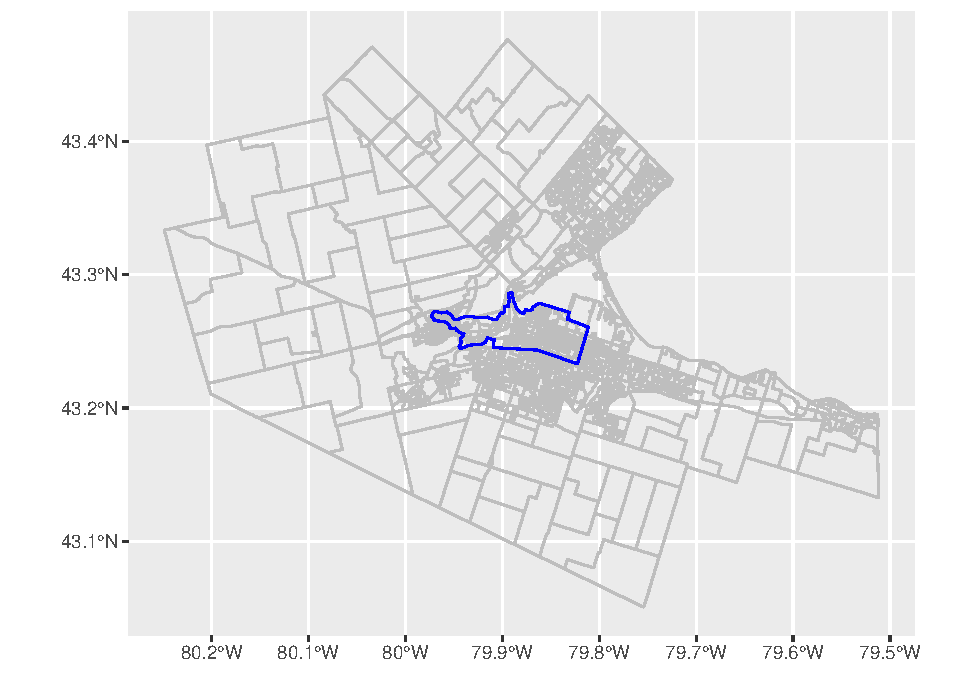
\includegraphics{Bike-share-spatial-equity_files/figure-latex/unnamed-chunk-4-1.pdf}

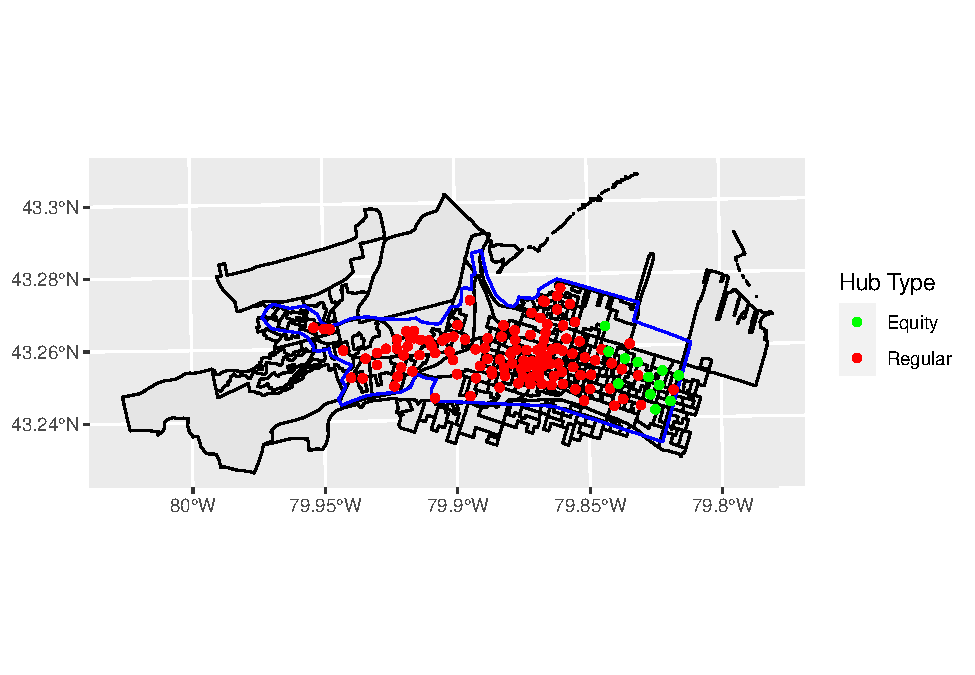
\includegraphics{Bike-share-spatial-equity_files/figure-latex/unnamed-chunk-6-1.pdf}

\hypertarget{methods}{%
\section{Methods}\label{methods}}

\hypertarget{results}{%
\section{Results}\label{results}}

\begin{enumerate}
\def\labelenumi{\arabic{enumi}.}
\item
  Accessibility (maps, descriptive statistics)
\item
  Comparison with and without ERI hubs (change in accessibility)
\item
\end{enumerate}

\hypertarget{discussion}{%
\section{Discussion}\label{discussion}}

Program achieved its stated goal to increase accessibility, only
modestly. It's an open question whether it changed behaviours.

Equity can be achieved in two different ways: equal spatial distribution
across a region (e.g., horizontal equity) or greater access to
vulnerable or disadvantaged populations (e.g., vertical equity)
({\textbf{???}}). By implementing ERI hubs in more disadvantaged areas
in Hamilton, the City of Hamilton has achieved greater horizontal equity
by extending the spatial distribution of bicycles across the city. But
our analysis found that vulnerable or disadvantaged populations do not
necessarily have greater access to the program.

\hypertarget{conclusion}{%
\section{Conclusion}\label{conclusion}}

\hypertarget{references}{%
\section*{References}\label{references}}
\addcontentsline{toc}{section}{References}


\end{document}


